% Shared standalone design for the editable figure reconstructions.
\documentclass[tikz,border=5pt,10pt]{standalone}
\usepackage[T1]{fontenc}
\usepackage[utf8]{inputenc}
\usepackage{newpxtext,newpxmath}
\usepackage[scaled=.94]{sourcesanspro}
\usepackage{pgfplots}
\pgfplotsset{compat=1.18}
\usetikzlibrary{arrows.meta,calc,positioning,decorations.pathreplacing,
  decorations.markings,patterns,matrix,shapes.geometric,fit,backgrounds,
  intersections,angles,quotes}
\definecolor{ink}{HTML}{203746}
\definecolor{accent}{HTML}{146C78}
\definecolor{muted}{HTML}{667780}
\definecolor{signalred}{HTML}{B94B44}
\color{ink}
\tikzset{>=Latex,line width=.8pt,
  every node/.style={font=\small},
  axis/.style={->,draw=muted,line width=.5pt},
  guide/.style={draw=muted,dashed,line width=.45pt},
  curve/.style={draw=accent,line width=1pt},
  marker/.style={circle,fill=accent,inner sep=1.5pt},
  labelbox/.style={fill=white,inner sep=2pt}}

\begin{document}
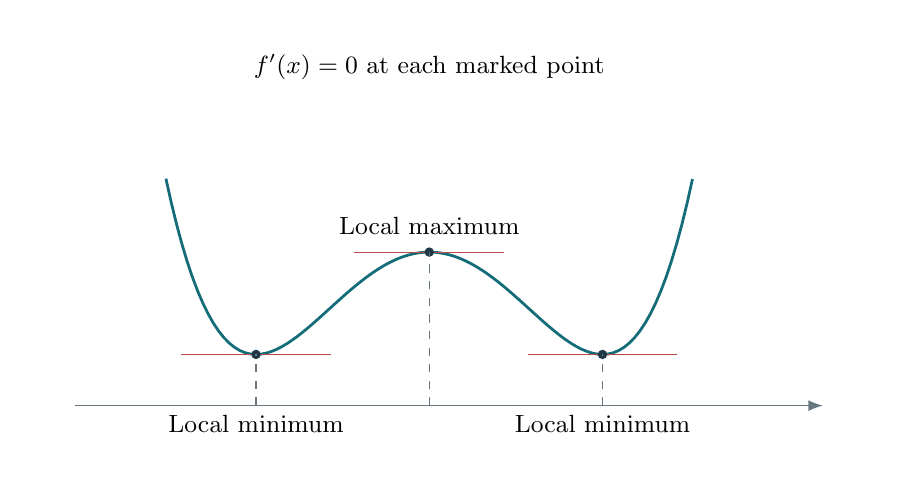
\begin{tikzpicture}
\path[use as bounding box] (-.6,-.6) rectangle (10.3,4.8);
\draw[axis] (0,0)--(9.5,0);
\begin{scope}[shift={(4.5,0)},xscale=2.2]
\draw[curve] plot[domain=-1.52:1.52,samples=101] (\x,{1.3*(\x*\x-1)^2+.65});
\end{scope}
\draw[signalred] (1.35,.65)--(3.25,.65) (3.55,1.95)--(5.45,1.95) (5.75,.65)--(7.65,.65);
\foreach \x/\y in {2.3/.65,4.5/1.95,6.7/.65}{\fill[ink] (\x,\y) circle (1.7pt);\draw[guide] (\x,0)--(\x,\y);}
\node[below] at (2.3,0) {Local minimum};\node[below] at (6.7,0) {Local minimum};
\node[above] at (4.5,2.05) {Local maximum};\node at (4.5,4.3) {$f'(x)=0$ at each marked point};
\end{tikzpicture}
\end{document}
